\chapter{用户上网数据采集与处理}
本章主要介绍用户上网如何留下信息,如何将用户上网信息转变为推荐系统所需要的训练集。其中包括了以下内容:网络信息通信协议及其结构、网页主要内容分布位置、网络流量信息采集、去除标签和过滤内容的策略、格式化、存储采集到信息的方法。

\section{网络信息通信协议及其结构}
互联网用户通过各类软件发送、接受信息。对于不同的软件,有不同的信息发送、接受格式,称作协议。以大多数网络浏览器使用的基本HTTP协议来说,其请求的头部有以下常用的信息 \\
\begin{center}
\tablecaption{HTTP协议请求头部常用的信息}
\label{table:HTTPinfo}
\begin{tabular}{l|p{10cm}}
 \hline
头部名称 & 描述 \\ \hline
回应接收类型 & 接受从对方服务器回应发来文件的类型 \\ \hline
请求内容类型 & 发送请求时请求主体的MIME类型(一般由POST请求或者PUT请求使用) \\ \hline
日期 & 发送信息时的日期与时间 \\ \hline
主服务器 & 服务器的域名(虚拟服务器)以及服务器所监听的TCP端口号(如果使用标准端口号,则忽略端口号) \\ \hline
引用源 & 前一个网页的地址(该网页上的链接到当前的网页) \\ \hline
用户代理 & 用户所使用的代理的信息(浏览器的信息等) \\
\hline
\end{tabular}
\end{center}

表\ref{table:HTTPinfo}简单介绍了HTTP协议请求头部中常用的信息。
根据HTTP请求头部我们可以获得用户请求网站URL,请求时间,使用浏览器类型信息。
通过网站URL可以简单将网页分为几类:
\begin{itemize}
\item 综合网页类。一些门户网站的首页通常含有各种关键词,所属范围较大,与用户的兴趣爱好没有多少关系,比如搜狐首页、新浪首页;
\item 搜索类网页。这些网页会包含一个或多个搜索关键词,并且这些关键词由用户输入,基本上能代表用户的兴趣爱好。例如在百度搜索等搜索引擎页面,通常会在其URL后接上搜索关键词的UTF-8编码;
\item 终点页面。这类网页通常包含一个或多个关键词,接着会有大篇幅文字描述相关内容。
\end{itemize}
根据以上分类可以为信息采集分类系统设计第一层过滤分类规则。
另外还能通过引用源的内容获取网页间的联系,经相互对比,增加网页信息抓取的准确度。

\section{网络内容采集}
仅通过分析网络请求与响应头部的信息,获取到的信息对于本系统来说远远不够。
所以需要记录并保存所有网络流量包,然后解压信息包,获得其中网页信息。
对于使用其他协议的软件来说,只要按照该协议的约定,也能正确解压信息包,获取其中内容。

\usetikzlibrary{backgrounds,calc,shadings,shapes.arrows,shapes.symbols,shadows}
\definecolor{switch}{HTML}{006996}
\makeatletter
\pgfkeys{/pgf/.cd,
  parallelepiped offset x/.initial=2mm,
  parallelepiped offset y/.initial=2mm
}
\pgfdeclareshape{parallelepiped}
{
  \inheritsavedanchors[from=rectangle] % this is nearly a rectangle
  \inheritanchorborder[from=rectangle]
  \inheritanchor[from=rectangle]{north}
  \inheritanchor[from=rectangle]{north west}
  \inheritanchor[from=rectangle]{north east}
  \inheritanchor[from=rectangle]{center}
  \inheritanchor[from=rectangle]{west}
  \inheritanchor[from=rectangle]{east}
  \inheritanchor[from=rectangle]{mid}
  \inheritanchor[from=rectangle]{mid west}
  \inheritanchor[from=rectangle]{mid east}
  \inheritanchor[from=rectangle]{base}
  \inheritanchor[from=rectangle]{base west}
  \inheritanchor[from=rectangle]{base east}
  \inheritanchor[from=rectangle]{south}
  \inheritanchor[from=rectangle]{south west}
  \inheritanchor[from=rectangle]{south east}
  \backgroundpath{
    % store lower right in xa/ya and upper right in xb/yb
    \southwest \pgf@xa=\pgf@x \pgf@ya=\pgf@y
    \northeast \pgf@xb=\pgf@x \pgf@yb=\pgf@y
    \pgfmathsetlength\pgfutil@tempdima{\pgfkeysvalueof{/pgf/parallelepiped
      offset x}}
    \pgfmathsetlength\pgfutil@tempdimb{\pgfkeysvalueof{/pgf/parallelepiped
      offset y}}
    \def\ppd@offset{\pgfpoint{\pgfutil@tempdima}{\pgfutil@tempdimb}}
    \pgfpathmoveto{\pgfqpoint{\pgf@xa}{\pgf@ya}}
    \pgfpathlineto{\pgfqpoint{\pgf@xb}{\pgf@ya}}
    \pgfpathlineto{\pgfqpoint{\pgf@xb}{\pgf@yb}}
    \pgfpathlineto{\pgfqpoint{\pgf@xa}{\pgf@yb}}
    \pgfpathclose
    \pgfpathmoveto{\pgfqpoint{\pgf@xb}{\pgf@ya}}
    \pgfpathlineto{\pgfpointadd{\pgfpoint{\pgf@xb}{\pgf@ya}}{\ppd@offset}}
    \pgfpathlineto{\pgfpointadd{\pgfpoint{\pgf@xb}{\pgf@yb}}{\ppd@offset}}
    \pgfpathlineto{\pgfpointadd{\pgfpoint{\pgf@xa}{\pgf@yb}}{\ppd@offset}}
    \pgfpathlineto{\pgfqpoint{\pgf@xa}{\pgf@yb}}
    \pgfpathmoveto{\pgfqpoint{\pgf@xb}{\pgf@yb}}
    \pgfpathlineto{\pgfpointadd{\pgfpoint{\pgf@xb}{\pgf@yb}}{\ppd@offset}}
  }
}
\makeatother

\tikzset{l3 switch/.style={
    parallelepiped,fill=switch, draw=white,
    minimum width=0.75cm,
    minimum height=0.75cm,
    parallelepiped offset x=1.75mm,
    parallelepiped offset y=1.25mm,
    path picture={
      \node[fill=white,
        circle,
        minimum size=6pt,
        inner sep=0pt,
        append after command={
          \pgfextra{
            \foreach \angle in {0,45,...,360}
            \draw[-latex,fill=white] (\tikzlastnode.\angle)--++(\angle:2.25mm);
          }
        }
      ] 
       at ([xshift=-0.75mm,yshift=-0.5mm]path picture bounding box.center){};
    }
  },
  ports/.style={
    line width=0.3pt,
    top color=gray!20,
    bottom color=gray!80
  },
  rack switch/.style={
    parallelepiped,fill=white, draw,
    minimum width=1.25cm,
    minimum height=0.25cm,
    parallelepiped offset x=2mm,
    parallelepiped offset y=1.25mm,
    xscale=-1,
    path picture={
      \draw[top color=gray!5,bottom color=gray!40]
      (path picture bounding box.south west) rectangle 
      (path picture bounding box.north east);
      \coordinate (A-west) at ([xshift=-0.2cm]path picture bounding box.west);
      \coordinate (A-center) at ($(path picture bounding box.center)!0!(path
        picture bounding box.south)$);
      \foreach \x in {0.275,0.525,0.775}{
        \draw[ports]([yshift=-0.05cm]$(A-west)!\x!(A-center)$)
          rectangle +(0.1,0.05);
        \draw[ports]([yshift=-0.125cm]$(A-west)!\x!(A-center)$)
          rectangle +(0.1,0.05);
       } 
      \coordinate (A-east) at (path picture bounding box.east);
      \foreach \x in {0.085,0.21,0.335,0.455,0.635,0.755,0.875,1}{
        \draw[ports]([yshift=-0.1125cm]$(A-east)!\x!(A-center)$)
          rectangle +(0.05,0.1);       
      }
    }
  },
  server/.style={
    parallelepiped,
    fill=white, draw,
    minimum width=0.35cm,
    minimum height=0.75cm,
    parallelepiped offset x=3mm,
    parallelepiped offset y=2mm,
    xscale=-1,
    path picture={
      \draw[top color=gray!5,bottom color=gray!40]
      (path picture bounding box.south west) rectangle 
      (path picture bounding box.north east);
      \coordinate (A-center) at ($(path picture bounding box.center)!0!(path
        picture bounding box.south)$);
      \coordinate (A-west) at ([xshift=-0.575cm]path picture bounding box.west);
      \draw[ports]([yshift=0.1cm]$(A-west)!0!(A-center)$)
        rectangle +(0.2,0.065);
      \draw[ports]([yshift=0.01cm]$(A-west)!0.085!(A-center)$)
        rectangle +(0.15,0.05);
      \fill[black]([yshift=-0.35cm]$(A-west)!-0.1!(A-center)$)
        rectangle +(0.235,0.0175);
      \fill[black]([yshift=-0.385cm]$(A-west)!-0.1!(A-center)$)
        rectangle +(0.235,0.0175);
      \fill[black]([yshift=-0.42cm]$(A-west)!-0.1!(A-center)$)
        rectangle +(0.235,0.0175);
    }  
  },
}

\usetikzlibrary{calc, shadings, shadows, shapes.arrows}

% Styles for interfaces and edge labels
\tikzset{%
  interface/.style={draw, rectangle, rounded corners, font=\LARGE\sffamily},
  ethernet/.style={interface, fill=yellow!50},% ethernet interface
  serial/.style={interface, fill=green!70},% serial interface
  speed/.style={sloped, anchor=south, font=\large\sffamily},% line speed at edge
  route/.style={draw, shape=single arrow, single arrow head extend=4mm,
    minimum height=1.7cm, minimum width=3mm, white, fill=switch!20,
    drop shadow={opacity=.8, fill=switch}, font=\tiny}% inroute/outroute arrows
}
\newcommand*{\shift}{1.3cm}% For placing the arrows later

% The router icon
\newcommand*{\router}[1]{
\begin{tikzpicture}    
  \coordinate (ll) at (-3,0.5);
  \coordinate (lr) at (3,0.5);
  \coordinate (ul) at (-3,2);
  \coordinate (ur) at (3,2);
  \shade [shading angle=90, left color=switch, right color=white] (ll)
    arc (-180:-60:3cm and .75cm) -- +(0,1.5) arc (-60:-180:3cm and .75cm)
    -- cycle;
  \shade [shading angle=270, right color=switch, left color=white!50] (lr)
    arc (0:-60:3cm and .75cm) -- +(0,1.5) arc (-60:0:3cm and .75cm) -- cycle;
  \draw [thick] (ll) arc (-180:0:3cm and .75cm)
    -- (ur) arc (0:-180:3cm and .75cm) -- cycle;
  \draw [thick, shade, upper left=switch, lower left=switch,
    upper right=switch, lower right=white] (ul)
    arc (-180:180:3cm and .75cm);
  \node at (0,0.5){\color{blue!60!black}\Huge #1};% The name of the router
  % The four arrows, symbols for incoming and outgoing routes:
  \begin{scope}[yshift=2cm, yscale=0.28, transform shape]
    \node[route, rotate=45, xshift=\shift] {\strut};
    \node[route, rotate=-45, xshift=-\shift] {\strut};
    \node[route, rotate=-135, xshift=\shift] {\strut};
    \node[route, rotate=135, xshift=-\shift] {\strut};
  \end{scope}
\end{tikzpicture}}

\makeatletter
\pgfdeclareradialshading[tikz@ball]{cloud}{\pgfpoint{-0.275cm}{0.4cm}}{%
  color(0cm)=(tikz@ball!75!white);
  color(0.1cm)=(tikz@ball!85!white); 
  color(0.2cm)=(tikz@ball!95!white); 
  color(0.7cm)=(tikz@ball!89!black); 
  color(1cm)=(tikz@ball!75!black)
}
\tikzoption{cloud color}{\pgfutil@colorlet{tikz@ball}{#1}%
  \def\tikz@shading{cloud}\tikz@addmode{\tikz@mode@shadetrue}}
\makeatother

\tikzset{my cloud/.style={
     cloud, draw, aspect=2,
     cloud color={gray!5!white}
  }
}
\begin{center}
\begin{tikzpicture}

\node[server](server 1){};
\node[server, right of= server 1](server 2){};
\node[server, right of= server 2](server 3){};

\node[rack switch, above of=server 2,xshift=0.1cm,yshift=0.3cm]
  (rack switch 1){};

\draw[thick,darkgray!10!gray] (server 1.north)--(rack switch 1);
\draw[thick,darkgray!10!gray] (server 2.north)--(rack switch 1);
\draw[thick,darkgray!10!gray] (server 3.north)--(rack switch 1);

\begin{scope}[xshift=3.5cm]
  \node[server](server 4){};
  \node[server, right of= server 4](server 5){};
  \node[server, right of= server 5](server 6){};

  \node[rack switch, above of=server 5,xshift=0.1cm,yshift=0.3cm]
  (rack switch 2){};

  \draw[thick,darkgray!10!gray] (server 4.north)--(rack switch 2);
  \draw[thick,darkgray!10!gray] (server 5.north)--(rack switch 2);
  \draw[thick,darkgray!10!gray] (server 6.north)--(rack switch 2);
\end{scope}

\begin{scope}[xshift=8cm]
  \node[server](server 7){};
  \node[server, right of= server 7](server 8){};
  \node[server, right of= server 8](server 9){};

  \node[rack switch, above of=server 8,xshift=0.1cm,yshift=0.3cm]
  (rack switch 3){};

  \draw[thick,darkgray!10!gray] (server 7.north)--(rack switch 3);
  \draw[thick,darkgray!10!gray] (server 8.north)--(rack switch 3);
  \draw[thick,darkgray!10!gray] (server 9.north)--(rack switch 3);
\end{scope}


\node[l3 switch, above of =rack switch 1, xshift=1.5cm,yshift=0.5cm]
  (l3 switch 1){};
\node[l3 switch, above of =rack switch 2, xshift=2cm,yshift=0.5cm]
  (l3 switch 2){};

\begin{scope}[very thick,darkgray!10!gray]
  \draw ($(rack switch 1.north)!0.5!(rack switch 1.north west)$)--
   ($(l3 switch 2.south)!0.5!(l3 switch 2.south west)$);
  \draw ($(rack switch 1.north)!0.5!(rack switch 1.north east)$)--
   ($(l3 switch 1.south)!0.5!(l3 switch 1.south west)$);

  \draw ($(rack switch 2.north)!0.5!(rack switch 2.north west)$)--
   ($(l3 switch 2.south)!0!(l3 switch 2.south west)$);
  \draw ($(rack switch 2.north)!0.5!(rack switch 2.north east)$)--
   ($(l3 switch 1.south)!0!(l3 switch 1.south west)$);  

  \draw ($(rack switch 3.north)!0.5!(rack switch 3.north west)$)--
   ($(l3 switch 2.south)!0.5!(l3 switch 2.south east)$);
  \draw ($(rack switch 3.north)!0.5!(rack switch 3.north east)$)--
   ($(l3 switch 1.south)!0.5!(l3 switch 1.south east)$); 

  \draw ($(l3 switch 2.north west)!0.25!(l3 switch 2.south west)$)--
  ($(l3 switch 1.north east)!0.25!(l3 switch 1.south east)$);

  \draw ($(l3 switch 2.north west)!0.75!(l3 switch 2.south west)$)--
  ($(l3 switch 1.north east)!0.75!(l3 switch 1.south east)$);

\end{scope} 

\node[l3 switch, above of =l3 switch 1, xshift=2cm,yshift=0.75cm](border 1){}; 

% = = = = = = = = = = = = = = = =
% Labels
% = = = = = = = = = = = = = = = =


\node[xshift=-1.05cm,yshift=0.2cm,left of = server 3,align=left](lev1)
  {User Devices};

\node[xshift=0.9cm,yshift=0.3cm,above of = lev1,align=left](lev2)
  {Access Layer};

\node[xshift=1.6cm,yshift=0.4cm,above of = lev2,align=left](lev3)
  {Aggregation Layer};
\node[xshift=2.55cm,yshift=0.75cm,above of = lev3,align=right](lev4)
  {Core Layer};
\node[xshift=-1cm,yshift=1.2cm,above of = lev4,align=right](lev5)
  {Gateway Router};
\node[xshift=7cm,yshift=0.1cm,above of = lev3,align=right](lev6)
  {Data captured here};
\node[xshift=7cm,yshift=-0.3cm,above of = lev3,align=right](lev7)
  {and analysed};

% = = = = = = = = = = = = = = = =
% Background rectangle - removed
% = = = = = = = = = = = = = = = =

\path ($(server 3.south west)!0.9!(lev1.south east)-(0,0.4cm)$) coordinate (A)
  --([yshift=0.86cm]A |- lev4.north east)coordinate (B)--
  ($(B)+(11.2cm,0)$)coordinate (C);

% = = = = = = = = = = = = = = = =
% Border Router and Internet
% = = = = = = = = = = = = = = = =

% interconnections of border 1
\begin{scope}[very thick,darkgray!10!gray]
  \draw ($(border 1.south)!0.5!(border 1.south west)$)--
   (l3 switch 1.north);

  \draw ($(border 1.south)!-0.5!(border 1.south west)$)--
   (l3 switch 2.north);
\end{scope}

\begin{scope}
  \node[yshift=1cm,xshift=-6cm,scale=0.2] (brouter) at (C) {\router{}}
    edge[very thick,darkgray!10!gray] ([xshift=0.1cm,yshift=0.5cm]border 1);

  \node[yshift=0.65cm,my cloud, minimum width=1.25cm, minimum height=1.55cm,
    above of=brouter,font=\large] (it) {Internet}
      edge[very thick,darkgray!30!gray] (brouter);
\end{scope}

\draw [dashed] (0,2.3) -- (5,2.3);
\draw [dashed] (0,5.3) -- (5,5.3);
\draw [dashed] (0,2.3) -- (0,5.3);
\draw [dashed] (5,2.3) -- (5,5.3);
\draw [->] (5,3.8) -- (7,3.8);
\node[server] at (7.5,3.8){};
\end{tikzpicture}
\figurecaption{用户数据采集及处理}
\label{fig:userinfocap}
\end{center}

在处理大量网络流量信息之前,可以先用小型工具抓取网络包进行分析。
Wireshark是一个跨平台的网络流量分析工具,能用于识别与分析多种网络协议包。
当网卡处于Promiscuous模式时,Wireshark能监听其所在局域网的所有网络包。
从Wireshark的GUI窗口可以简明地查看包信息,以及解压包获取其中内容。
Wireshark还能设置强大的过滤条件,从而筛选出目标网络包。
Wireshark适用于Windows平台用户,对于使用Linux的用户而言,可以使用Iptables完成上述分析步骤。

对于大型的路由器或交换网络的情况,如图\ref{fig:userinfocap}中的多层级网络,Wireshark和Iptables就不太适用。
目前,国内外比较流行使用的大型网络流量信息采集方式有Cisco公司开发的NetFlow工具。
支持NetFlow的路由器和交换机能够收集所有接口上IP交换数据,并且能把数据导出到NetFlow信息分析服务器上。
国内研究人员也设计了类似的分布式网络流量分析系统\parencite{乔媛媛2014基于,延皓2011基于流量监测的网络用户行为分析,董超2013基于网络流量监测的移动互联网特征研究}。

本文根据NetFlow采集模式设计采集及处理模块,如图\ref{fig:userinfocap}所示。
对于每个地区的路由器或者交换机,都连接到信息分析服务器。
信息分析服务器将对文件的Content-Type进行过滤。
目前,包含有效信息的网络文件类型大部分为HTML,另外还有一部分内容通过JSON文件与XML文件传输。
但是随着Javascript的极速发展,相当一部分HTML由浏览器从Javascript文件中生成,即网络内容不再是显式传输,而是隐藏在JSON文件与XML文件中,填充到Javascript生成的HTML框架中。
这对本文的网页信息分析造成了一定的困难。
经过简单的过滤,可以记录保存表\ref{table:infoformatone}中标定的信息。
\begin{center}
\tablecaption{信息分析服务器记录信息格式}
\label{table:infoformatone}
\begin{tabular}{c|c|c|c|c|c}
	\hline
	User ID & Request URL & Time & Location & Content & Device \\
	\hline
\end{tabular}
\end{center}

\section{网络信息处理及分类}
通过前两节的分析,混杂的网络信息已经归档为按表\ref{table:infoformatone}中格式的记录。
为处理和分类这些有序信息,本节形成策略如图\ref{fig:classify}:
\usetikzlibrary{%
  arrows,%
  shapes.misc,% wg. rounded rectangle
  shapes.arrows,%
  chains,%
  matrix,%
  positioning,% wg. " of "
  scopes,%
  decorations.pathmorphing,% /pgf/decoration/random steps | erste Graphik
  shadows%
}
\tikzset{
  nonterminal/.style={
    % The shape:
    rectangle,
    % The size:
    minimum size=6mm,
    % The border:
    very thick,
    draw=red!50!black!50,         % 50% red and 50% black,
                                  % and that mixed with 50% white
    % The filling:
    top color=white,              % a shading that is white at the top...
    bottom color=red!50!black!20, % and something else at the bottom
    % Font
    font=\itshape
  },
  terminal/.style={
    % The shape:
    rounded rectangle,
    minimum size=6mm,
    % The rest
    very thick,draw=black!50,
    top color=white,bottom color=black!20,
    font=\ttfamily},
  skip loop/.style={to path={-- ++(0,#1) -| (\tikztotarget)}}
}

{
  \tikzset{terminal/.append style={text height=1.5ex,text depth=.25ex}}
  \tikzset{nonterminal/.append style={text height=1.5ex,text depth=.25ex}}
}
\begin{center}
\begin{tikzpicture}[
        point/.style={coordinate},>=stealth',thick,draw=black!50,
        tip/.style={->,shorten >=0.007pt},every join/.style={rounded corners},
        hv path/.style={to path={-| (\tikztotarget)}},
        vh path/.style={to path={|- (\tikztotarget)}},
        text height=1.5ex,text depth=.25ex % align text horizontally
    ]
    \scriptsize
    \matrix[column sep=4mm] {
        \node (p1) [point] {}; & \node (zhuabao) [nonterminal] {抓包};     &
        \node (p2) [point] {}; & \node (html)    [terminal]    {HTML文件};        &
        \node (p3) [point] {}; &                                              &
        \node (p4) [point] {}; & \node (getridoftag) [nonterminal] {去除标签}; &
        \node (p5) [point] {}; & \node (diyilei)   [terminal]    {综合网页};   &
        \node (p6) [point] {}; & \node (yuyifenxi) [nonterminal] {语义分析}; &
        \node (p7) [point] {}; \\
        % Third row:
        & & & \node (xml) [terminal] {XML文件}; & & &  & & & \node (dierlei) [terminal] {搜索网页}; & & & \\
        & & & \node (javascript) [terminal] {Javascript}; & \node (p8) [point] {}; & \node (javascriptvm) [nonterminal] {Javascript模拟器}; &  & & & \node (disanlei) [terminal] {终点网页}; & & & \\
        & & & \node (json)    [terminal]    {Json文件}; & & &  & & & & & & \\
    };

    { [start chain]
        \chainin (p1);
        \chainin (zhuabao)   [join=by tip];
        \chainin (p2)    [join];
        { [start branch=xml]
        \chainin (xml) [join=by {vh path,tip}];
        \chainin (p8)    [join=by {hv path}];
        }
        { [start branch=javascript]
        \chainin (javascript) [join=by {vh path,tip}];
        \chainin (p8)    [join];
        }
        { [start branch=json]
        \chainin (json) [join=by {vh path,tip}];
        \chainin (p8)    [join=by {hv path}];
        \chainin (javascriptvm) [join=by tip];
        \chainin (p4)    [join=by {hv path}];
        }

        \chainin (html)   [join=by tip];
        \chainin (p3)    [join];
        \chainin (p4)    [join];

        \chainin (getridoftag) [join=by tip];
        \chainin (p5)    [join];
        { [start branch=dierlei]
        \chainin (dierlei)  [join=by {vh path,tip}];
        \chainin (p6)    [join=by {hv path,tip}];
        }
        { [start branch=disanlei]
        \chainin (disanlei) [join=by {vh path,tip}];
        \chainin (p6)    [join=by {hv path,tip}];
        }
        \chainin (diyilei)    [join=by tip];
        \chainin (p6)     [join];
        \chainin (yuyifenxi)    [join=by tip];
        \chainin (p7)    [join=by tip];
    }
\end{tikzpicture}
\normalsize
\figurecaption{网页信息处理分类策略}
\label{fig:classify}
\end{center}
该策略的主要描述如下:网页信息处理分类首先将表\ref{table:infoformatone}中的网络协议包解压,
然后获得HTML文件,或者Javascript文件与XML文件、JSON文件。
将后三者放入Javascript虚拟机中,可以生成HTML文件。
接着按照HTML文件的请求URL或者标题内容进行分类,
按前一节所描述的网页分类分为综合网页,搜索网页或者终点网页。
由于URL包含网站名称,以及访问路径,故URL包含部分关键词,可将URL作为一个语句进行语义分析。
另外,由于HTML文件结构可知,其中的内容镶嵌在各种HTML标签中。
故分析HTML文件首先要去除各种标签。
通过实现监督学习算法\parencite{Kohlsch2010Boilerplate}去除标签,将剩下的文字内容输入语义分析模块。
最后,按网页类型做不同分析重点的语义分析。

按照第二章第一节描述的语义分析原理,本模块处理网页,分析得出所有关键词。
从关键词中取出所有名词,并按照出现次数进行排序。
将高频名词按照表\ref{table:infoformattwo}格式输出保存。
\begin{center}
\tablecaption{信息分析服务器输出信息格式}
\label{table:infoformattwo}
\begin{tabular}{c|c|c|c|c|c}
	\hline
	User ID & Request URL & Time & Location & Item & Device \\
	\hline
\end{tabular}
\end{center}

\section{在Hadoop上实现基于用户历史的协同过滤算法}
根据Hadoop与MapReduce的原理及特点,我们可以将基于用户历史的协同过滤算法计算过程分解到Map阶段与Reduce阶段中。

首先要进行简单的计数工作,即计算每个User-Item对的数目。
将该数目代入逻辑函数$S(t)=1/(1+e^{-t})$进行简单的归一化。
得到User-Item-Value格式的一组数据,形成下一步所需的User-Item矩阵,记为$R=\{<i,j,r_{i,j}>\}$,保存于Hadoop的HDFS中。
以下假设$n$个用户,$m$个物品,

\subsection{计算每个用户的平均评分}
每个用户$i$的平均评分可以如下计算:
\begin{equation}
\bar{r_i} = \frac{\sum_{j=1}^n r_{i,j}}{\sum_{k=1}^l 1}\qquad \forall i\in [1,n]
\end{equation}
其中$l$表示该用户评价了几个物品。

生成的平均评分数据集记为$U_{all}=\{<i,\bar{r}_i>\},\forall i\in [1,n]$。具体的Map与Reduce算法如下:
\begin{itemize}
\item Map-I:将$i$相同的$<i,j,r_{i,j}>$映射到同一个机器中,简记为$<j,r_{i,j}>$。
对于$k$个机器,本步骤的复杂度为$o(\frac{nm}{k})$。
\item Reduce-I:取出$<i,j,r_{i,j},\bar{r}_i>$,保存到HDFS中,此时将$R$指向$\{<i,j,r_{i,j},\bar{r}_i>\}$。
另外保存$U_{all}=\{<i,\bar{r}_i>\},\forall i\in [1,n]$到HDFS中。
本步骤的复杂度同样为$o(\frac{nm}{k})$。
\end{itemize}

\subsection{计算用户间相似度}
计算用户间相似度矩阵$S={S_{i,j}|\forall i,j\in[1,n]}$。
定义$U_i = \{<i,j,r_{i,j},\bar{r}_i>|\forall j \in [1,m],<i,j,r_{i,j},\bar{r}_i>\in R\}$为用户$i$评价过的物品集。
定义$N_{k,l} = U_k \cap U_l$,为用户$k$与用户$l$共同评价过的物品集。
为了计算可行性,$N_{k,l}$将分到同一个节点上。具体的Map与Reduce算法如下:
\begin{itemize}
\item Map-II:将$\{U_i|i\in [1,n]\}$映射为$\{N_i,j|\forall i,j\in [1,n]\}$。
如果有$k$个机器,本步骤的复杂度为$o(\frac{m^2n}{k})$。
\item Reduce-II:取出$\{S_{i,j}|\forall i,j\in [1,n]\}$,保存到HDFS中。
本步骤的复杂度为$o(\frac{m^2n}{k})$。
\end{itemize}
此步骤可以看出可以看出,对于物品数远大于用户数的情况,本算法更适合于用户数远大于物品数的情况。

\subsection{计算预测矩阵}
将矩阵$R$变形为矩阵$I$,其中矩阵$I$的数据按物品的序号排序:
\begin{equation}
I=\left(
\begin{array}{c}
I_1 \\
I_2 \\
\vdots \\
I_m
\end{array}
\right) = \{I_j|\forall j\in [1,m] \}
\end{equation}
其中
\begin{equation}
I_j=\left(
\begin{array}{c}
<1,j,r_{1,j},\bar{r}_1 > \\
<2,j,r_{2,j},\bar{r}_2 > \\
\vdots \\
<n,j,r_{n,j},\bar{r}_n >
\end{array}
\right) = \{<i,j,r_{i,j},\bar{r}_i >|\forall i\in [1,n], <i,j,r_{i,j},\bar{r}_i > \in R\}
\end{equation}
即$I_j$表示与物品$j$相关的所有评分数据集。
定义相似度矩阵$S$为
\begin{equation}
S=\left(
\begin{array}{ccc}
S_{1,1} & \ldots & S_{1,n} \\
\vdots & \vdots & \vdots \\
S_{n,1} & \ldots & S_{n,n} \\
\end{array}
\right) = \left(
\begin{array}{c}
S_1 \\
\vdots\\
S_n
\end{array}
\right)
\end{equation}
其中$S_i=\{S_{i,j}|\forall j\in [1,n] \}$表示用户$i$与其它用户间的相似度。
具体的Map与Reduce算法如下:
\begin{itemize}
\item Map-III:将$j$相同的$<i,j,r_{i,j}>$映射到同一个机器中,简记为$<j,r_{i,j}>$,同时将$S_i$映射到同一个机器中。
对于$k$个机器,本步骤的复杂度为$o(\frac{nm}{k})$。
\item Reduce-III:取出$B=<i,j,r_{i,j},\bar{r}_i ,S_i>$,保存到HDFS中。
本步骤的复杂度为$o(\frac{m^2n}{k})$。
\end{itemize}
这一步是为计算预测矩阵做准备。按照第二章的公式计算用户$i$对物品$j$的评分$p_{i,j}$。预测矩阵$P$定义为:
\begin{equation}
P=\left(
\begin{array}{c}
 \{ p_{1,1},p_{1,3},p_{1,5} \} \\
\vdots \\
\{ p_{i,1},p_{i,3},p_{i,5} \} \\
\vdots \\
\{p_{n,1},p_{n,3},p_{n,5}\}
\end{array}
\right) = \left(
\begin{array}{c}
P_1 \\
\vdots\\
P_i\\
\vdots \\
P_n
\end{array}
\right)
\end{equation}
其中$P_i=\{p_{i,j}|\forall j\in [1,m],<i,j,r_{i,j},\bar{r}_i>\notin R\},\forall i\in[1,n]$表示用户$i$对未评价物品集的所有预测分数。
具体的Map与Reduce算法如下:
\begin{itemize}
\item Map-IV:将$i$相同的$B=<i,j,r_{i,j},\bar{r}_i ,S_i>$映射到同一个机器中,简记为$<j,r_{i,j},\bar{r}_i ,S_i>$,同时将Map-I生成的$U_{all}$中的$U_i$映射到同一个机器中。对于$k$个机器,本步骤的复杂度为$o(\frac{nm}{k})$。将
\item Reduce-IV:取出$P=<i,j,p_{i,j},>$,保存到HDFS中。本步骤的复杂度为$o(\frac{m^2n}{k})$。
\end{itemize}
至此所有用户对未评价物品集的分数$p_{i,j}$都已经计算出来。
即构建了完整的User-Item矩阵,也即用户兴趣模型。
此时对于每个用户,对所有物品按评价分数大小排序,排名前k的物品组成一个向量。
下一步可以根据这个向量推荐用户内容。

\section{在Hadoop上实现基于模型的协同过滤算法}
在上一章中已经具体解释了,交替最小方差算法更适合于在Hadoop上实现的基于模型的协同过滤算法。

对于交替最小方差算法,主要步骤是矩阵$R$与矩阵$M$和矩阵$U$之间的联合操作。
通常来说,User-Item矩阵$R$要远远大于特征矩阵。
但是,本文只考虑矩阵$M$和矩阵$U$都不需要切分,即矩阵$M$和矩阵$U$都能保存在单个运算节点的内存中,的情况下,实现具体算法。

初步估计在并行计算的过程中,需要max$(|C|,|P|)\times r \times 8$个字节的内存量。
对于1千万数量级的用户数或者物品数,特征数为100的情况,大概需要8GB的内存,就目前的计算机水平,这个条件很容易满足。

基于以上设定,下面介绍交替最小方差算法的具体步骤。
首先从用户数据集$U$或者物品数据集$M$中取相对小的一个,复制到集群的每个计算节点中。
另外每个计算节点本地都有User-Item矩阵$R$的副本。
然后,通过一个map运算,把矩阵$R$的副本和矩阵$M$结合起来(矩阵$R$的副本和矩阵$U$类似)。
另外,在这个map运算中,我们还能从结合的结果实现中并行计算特征向量的逻辑,也就是说,我们可以在单独一个map运算中,运行一整套矩阵$U$和矩阵$M$的计算。
\begin{center}
\def\Machineone{
  \draw[rounded corners=1ex,color=blue!20!,fill=blue!20!] (0,0) rectangle (3,3);
  \draw[rounded corners=1ex,fill=white] (0.5,2) rectangle (2.5,2.5);
  \draw[fill=gray] (0.5,0.5) rectangle (1.8,1.5);
  \draw[fill=gray] (1,3.5) rectangle (2,4.5);
  \draw[->] (1.15,1.5) -- (1.15,2);
  \draw[->] (1.5,3) -- (1.5,3.5);
  \node at (1.5,2.25) {\textbf{Map}};
  \node at (1.15,1) [white] {$A(1)$};
  \node at (1.55,4) [white] {$U(1)$};
  \node at (1.5,-0.5) {Machine 1};
}
\def\Machinetwo{
  \draw[rounded corners=1ex,color=blue!20!,fill=blue!20!] (0,0) rectangle (3,3);
  \draw[rounded corners=1ex,fill=white] (0.5,2) rectangle (2.5,2.5);
  \draw[fill=gray] (0.5,0.5) rectangle (1.8,1.5);
  \draw[fill=gray] (1,3.5) rectangle (2,4.5);
  \draw[->] (1.15,1.5) -- (1.15,2);
  \draw[->] (1.5,3) -- (1.5,3.5);
  \node at (1.5,2.25) {\textbf{Map}};
  \node at (1.15,1) [white] {$A(2)$};
  \node at (1.55,4) [white] {$U(2)$};
  \node at (1.5,-0.5) {Machine 2};
}
\def\Machinethree{
  \draw[rounded corners=1ex,color=blue!20!,fill=blue!20!] (0,0) rectangle (3,3);
  \draw[rounded corners=1ex,fill=white] (0.5,2) rectangle (2.5,2.5);
  \draw[fill=gray] (0.5,0.5) rectangle (1.8,1.5);
  \draw[fill=gray] (1,3.5) rectangle (2,4.5);
  \draw[->] (1.15,1.5) -- (1.15,2);
  \draw[->] (1.5,3) -- (1.5,3.5);
  \node at (1.5,2.25) {\textbf{Map}};
  \node at (1.15,1) [white] {$A(3)$};
  \node at (1.55,4) [white] {$U(3)$};
  \node at (1.5,-0.5) {Machine 3};
}

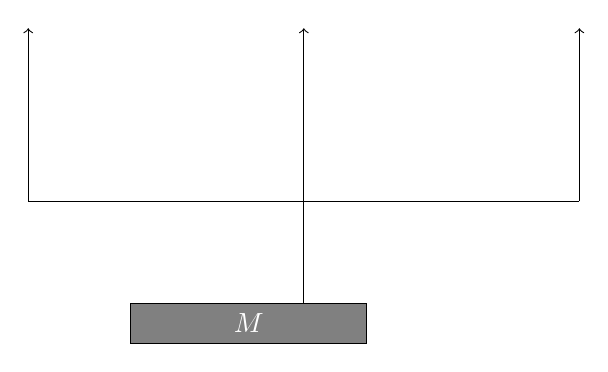
\begin{tikzpicture}
\Machineone
\begin{scope}[xshift=3.5cm]
\Machinetwo
\end{scope}
\begin{scope}[xshift=7cm]
\Machinethree
\end{scope}
\draw[fill=gray] (3.5,-2) rectangle (6.5,-1.5);
\draw[->] (5.7,-1.5) -- (5.7,2);
\draw[-] (2.2,-0.2) -- (9.2,-0.2);
\draw[->] (2.2,-0.2) -- (2.2,2);
\draw[->] (9.2,-0.2) -- (9.2,2);
\node at (5,-1.75) [white] {$M$};
\end{tikzpicture}
\figurecaption{基于模型的协同过滤算法MapReduce实现}
\label{fig:CFMap}
\end{center}
图\ref{fig:CFMap}描述了在三个计算节点上计算矩阵$U$时的并行结合方法。
我们将矩阵$M$分发到每个计算节点中,然后计算节点会给矩阵$M$的特征向量创建一个哈希表。
保存在HDFS中的矩阵$R$按行分块储存,并作为map运算的输入。
$R(1)$代表矩阵$R$的第一个分块。
接着,map运算读入矩阵$R$其中一行$r_i$然后选择其中部位零的下标,按照这些下标从哈希表找到矩阵$M$中对应的$m_j$。
然后,map运算将解一个线性方程,这个线性方程由交互信息$r_i$和物品特征向量$m_j$构成。
在得到方程解后,将结果写入HDFS中。
对于矩阵$M$的计算,其计算步骤类似,唯一的不同点在于,要在每个运算节点分发矩阵$U$,以及按照列来对矩阵$R$进行分块储存。

以上的计算方法只使用了map运算,因为相对于map运算与reduce运算一起使用,单独使用map运算在时间安排上更加灵活。
另外,我们还避免使用耗时很长的混排阶段,因为在混排阶段,大量数据要通过速率不太高的网络进行传输。
由于我们能够在一次map运算中运行矩阵结合以及计算的步骤,所以矩阵结合的结果就没必要写到HDFS中。
在计算线性方程的初始化阶段,我们通过Hadoop的分布式缓存分发特征矩阵。
另外,我们将Hadoop设置为在工作节点上重用虚拟机,并把特征向量矩阵缓存在内存中以避免接下来的map函数要重新读取数据。


